\documentclass[a4paper]{article}

\usepackage[utf8]{inputenc}
\usepackage[margin=1in]{geometry}
\usepackage[bookmarks]{hyperref}
\usepackage{graphicx}
\usepackage{listings}
\usepackage{color}
\usepackage{pdfpages}
\usepackage[style=verbose]{biblatex}
\usepackage{filecontents}
\usepackage{fancyref}
\usepackage[super]{nth}
\usepackage{siunitx}
\usepackage[inline]{enumitem}

\def \IPF {\texttt{IPv4}}
\def \IPS {\texttt{IPv6}}

\author{Huw Jones\\27618153\\hcbj1g15@soton.ac.uk}
\title{COMP2207: Distributed Systems and Networks}
\def \subtitle {IPv4/IPv6 Performance Report}


\hypersetup{
  pdfinfo={ee
    Title={\@title},
    Subtitle={\@subtitle}
    Author={\@author},
  },
  colorlinks=false,
  pdfborder=0 0 0,
}

\begin{filecontents}{bib.bib}
@online{ip_location,
  title = {IP Location Finder - Geolocation},
  url = {https://iplocation.net}
}
\end{filecontents}
\addbibresource{bib.bib}
\pagestyle{headings}

\begin{document}
\makeatletter
\begin{titlepage}
	\centering
	{\scshape\LARGE University of Southampton \par}
	\vspace{2cm}
    {\huge\bfseries \@title \par}
    \vspace{1cm}
	{\scshape\huge \subtitle \par}
	\vspace{3cm}
    {\Large
    \begin{tabular}{c}
      \@author
    \end{tabular} \\}
  \vspace{6cm}
    {\Large
    \today
    }
\end{titlepage}
\makeatother
\newpage

%%
%% SECTION: Data Gathering
%%
\section{Data Gathering}
To gather the data, I decided to create a bash script.
The idea was to use the native \texttt{ping} and \texttt{ping6} commands available in standard POSIX compatible environments to do the actual pinging,
and then use the standard utilities to save the min/max/average/standard deviation data into a CSV file (along with the time and IP that was pinged).

My script had options to specify the number of pings and interval between pings.
I used bash's inbuilt \texttt{getopts} using flags in order to set these values.
I defaulted to setting the number of pings to 30 and the interval to 0.5 seconds.
This meant each test would take a minimum of 15 seconds and therefore each running of the script would take on average 25 to 30 minutes.

My script logged the time of day, the IP address (resolved from the hostname) and then min/max/average/standard deviation.
It logged the data independently for each host.
This meant each host's IPv4 and IPv6 data was kept in different files and therefore kept separate.
I chose to log this much data as it would give greater flexibility later when analysing the results.

I left my data gathering script running for about a day on two servers.
The first was the UG Login server (\texttt{uglogin.ecs.soton.ac.uk}: \texttt{152.78.71.152}, \texttt{2001:630:d0:f110:250:56ff:fea0:7d2}) which supports \IPF/\IPS.
The second is my own website/droplet (\texttt{huwcbjones.co.uk}: \texttt{46.101.18.128}, \texttt{2a03:b0c0:1:d0::9b:e001}) which also supports \IPF/\IPS.

It is important to note, that after data collection, I manually went through and removed anomalous results from my dataset.
These were results where there was an odd one or even two ping results that were a few orders of magnitude slower than all the other results I gathered.
I removed these results as they were anomalous and skewed my averages much higher than should have been expected.

I then wrote another quick bash script, \texttt{summary.sh}, to extract the hostname, minimum ping, maximum ping, status (success, blocked, no route)
  and calculate the overall average ping time.
This left me with a \texttt{summary.4.csv} file and a \texttt{summary.6.csv} file containing each host and the average ping from both servers.
I then combined these four files together along with the \texttt{Top100Sites.csv} in excel to produce a table of:
rank, hostname, Minimum {\IPF} Ping, Maximum {\IPF} ping, Average {\IPF} ping, Minimum {\IPS} Ping, Maximum {\IPS} ping and average {\IPS} ping.

My script did not actively cater for sites that either blocked pings, or were not accessible (no route).
But by chance, the data was able to be differentiated.
Sites that were not accessible left blanks in the entries, and sites that blocked the pings left `\textit{100\% packet failure}'.
My \texttt{summary.sh} script was able to differentiate this when producing the summaries.

%%
%% SECTION: Results
%%
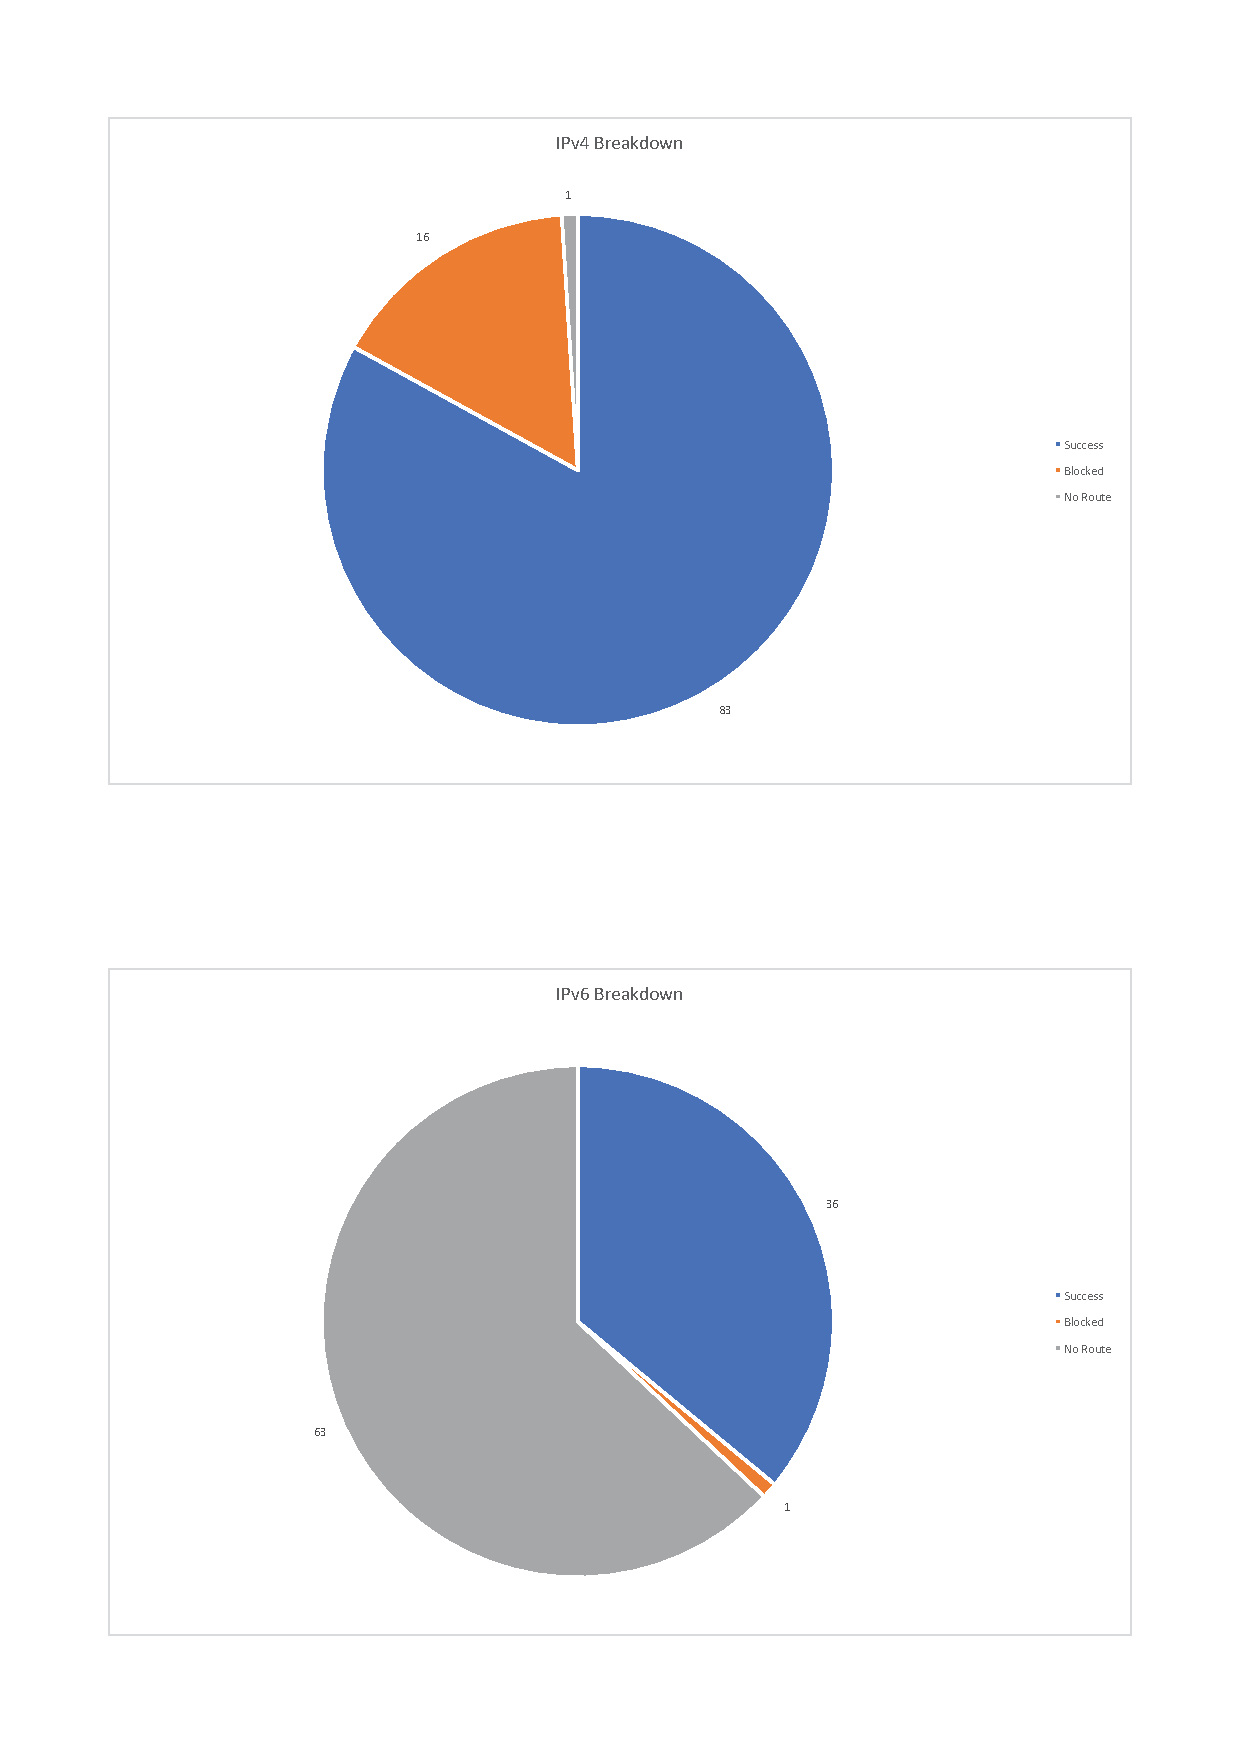
\includepdf[landscape=false,scale=0.9,pagecommand={\section{Results}\subsection{{\IPF/\IPS} Breakdown}\label{sec:res_breakdown}}]{charts/Breakdown.pdf}
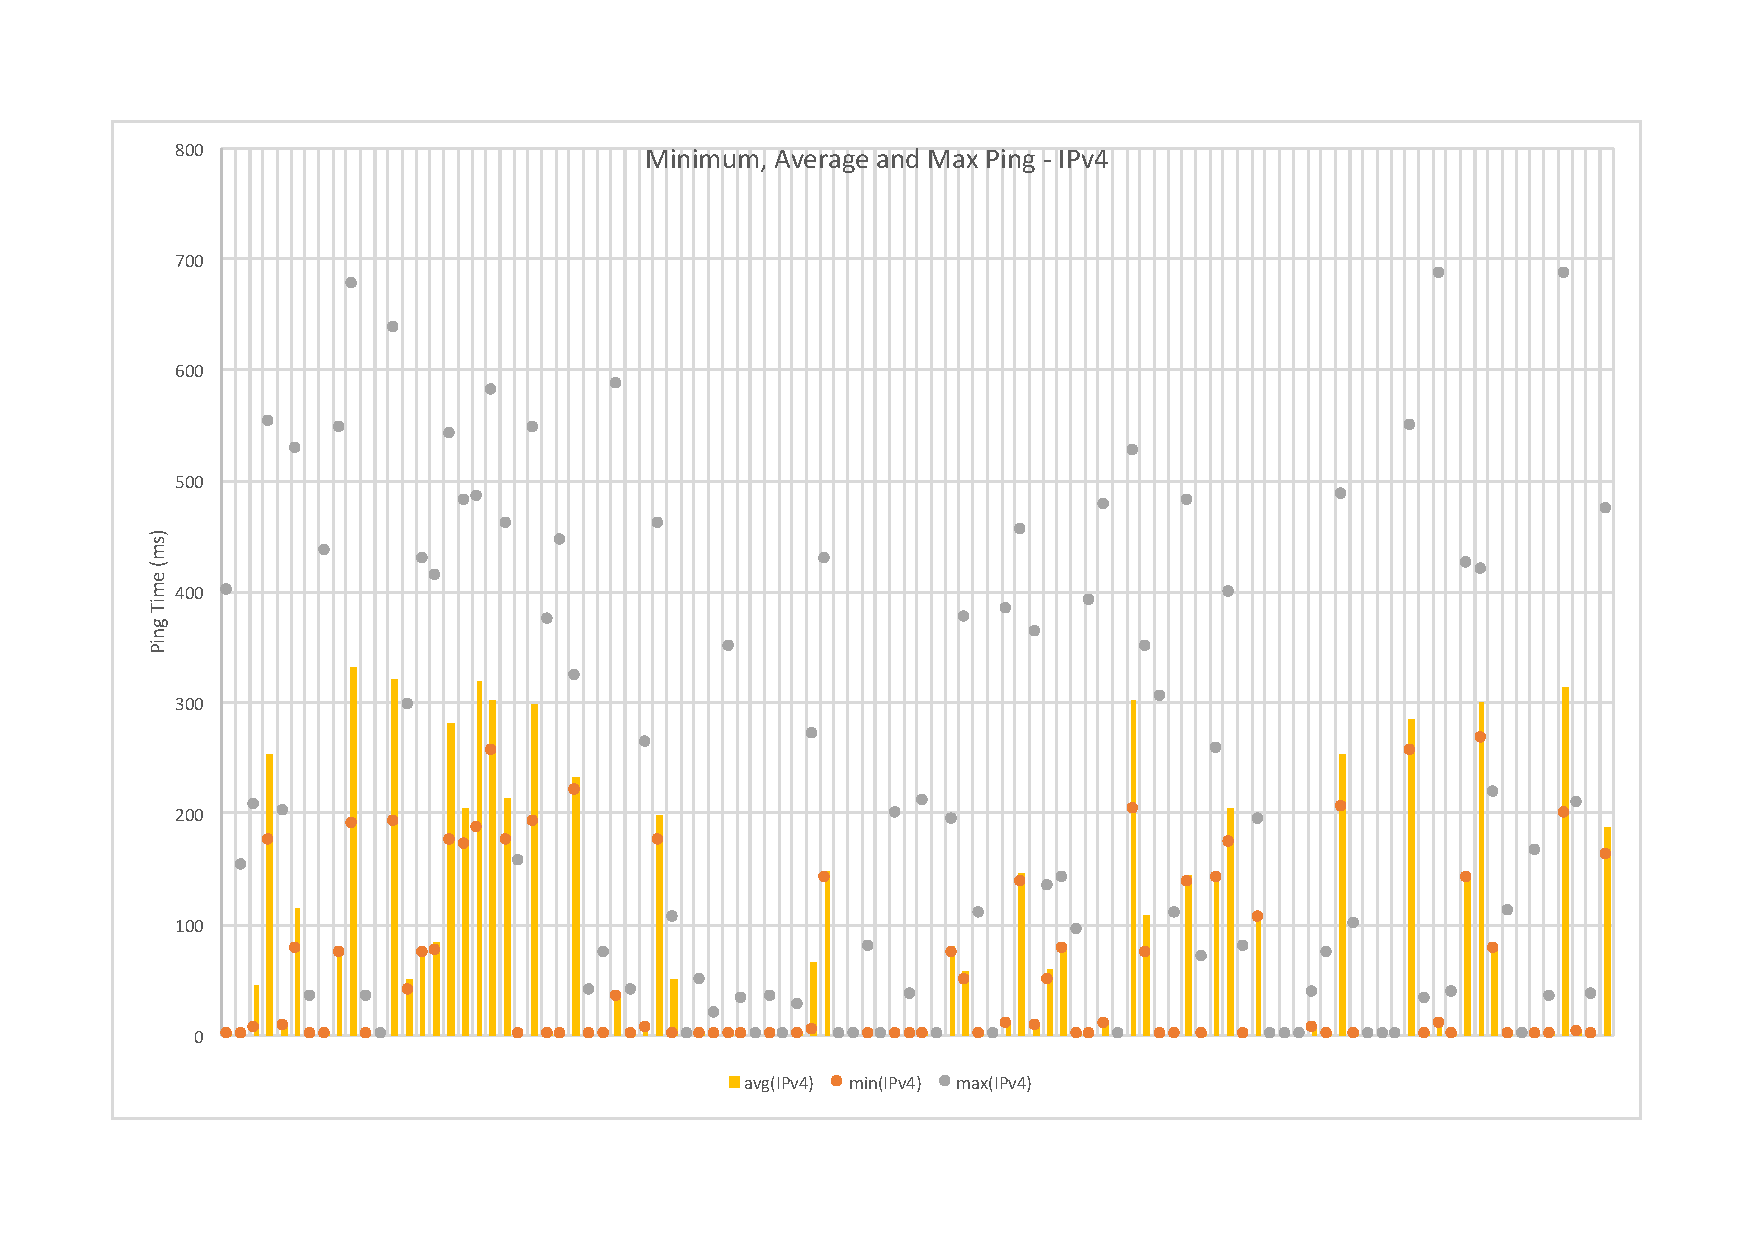
\includepdf[landscape=false,scale=0.9,angle=90,pagecommand={\subsection{{\IPF} Statistics}\label{sec:res_ipv4}}]{charts/IPv4_Stats.pdf}
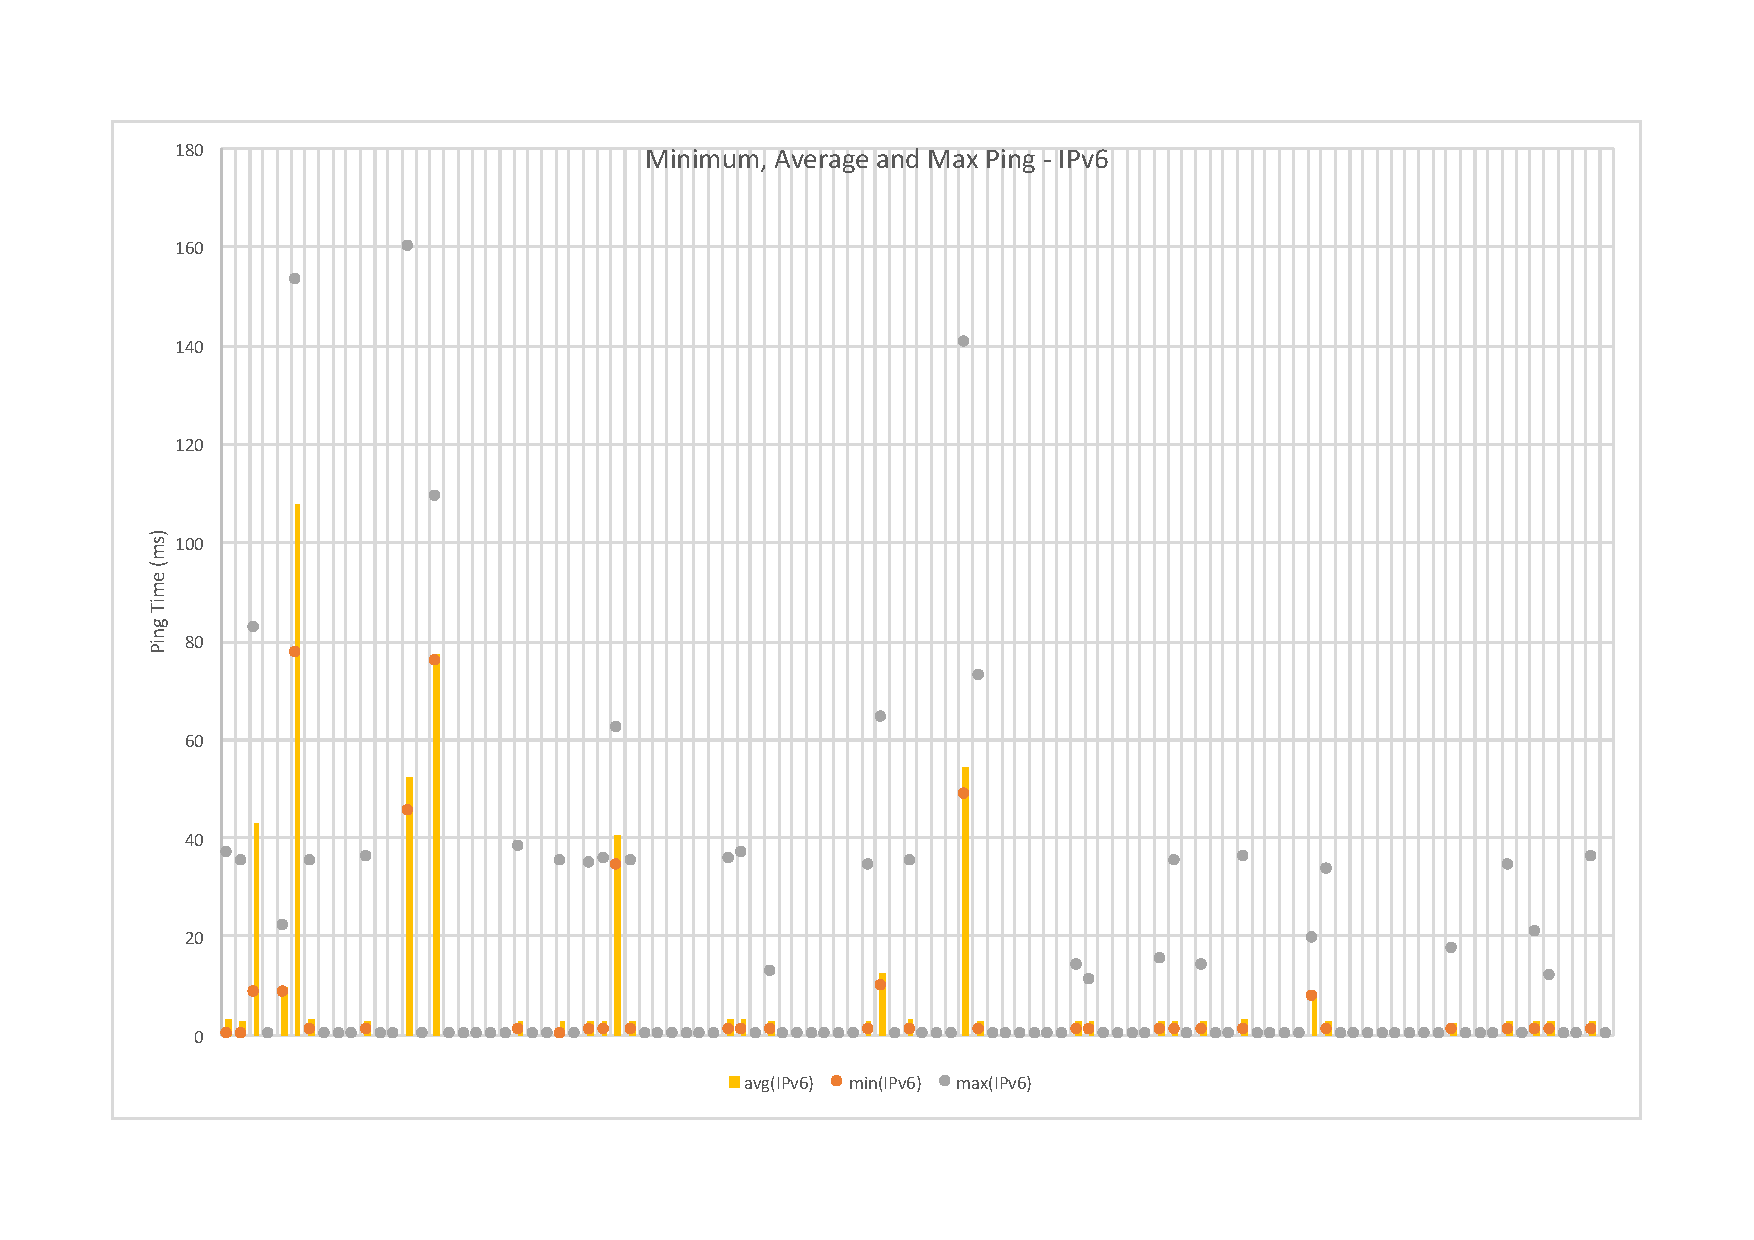
\includepdf[landscape=false,scale=0.9,angle=90,pagecommand={\subsection{{\IPS} Statistics}\label{sec:res_ipv6}}]{charts/IPv6_Stats.pdf}
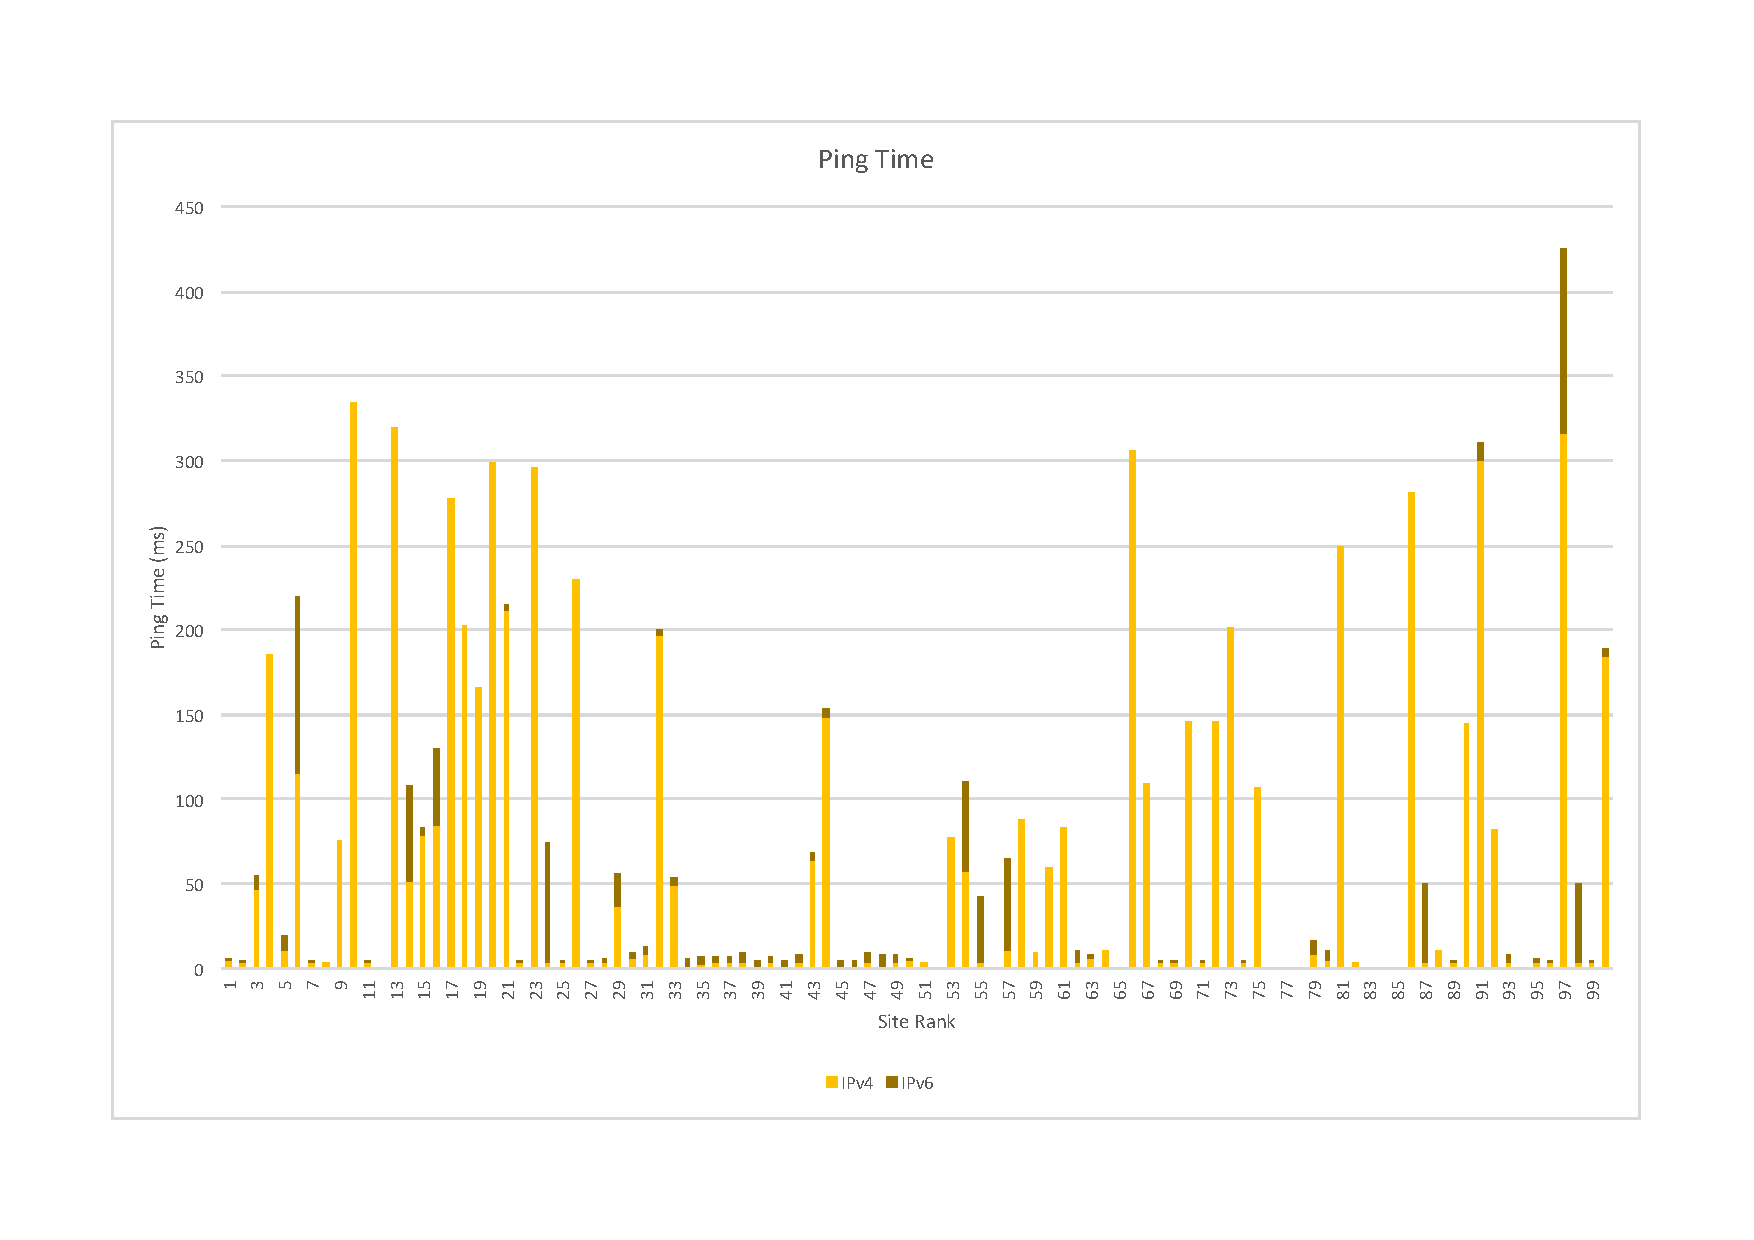
\includepdf[landscape=false,scale=0.9,angle=90,pagecommand={\subsection{Ping Time Stacked}}\label{sec:res_stacked}]{charts/stacked.pdf}
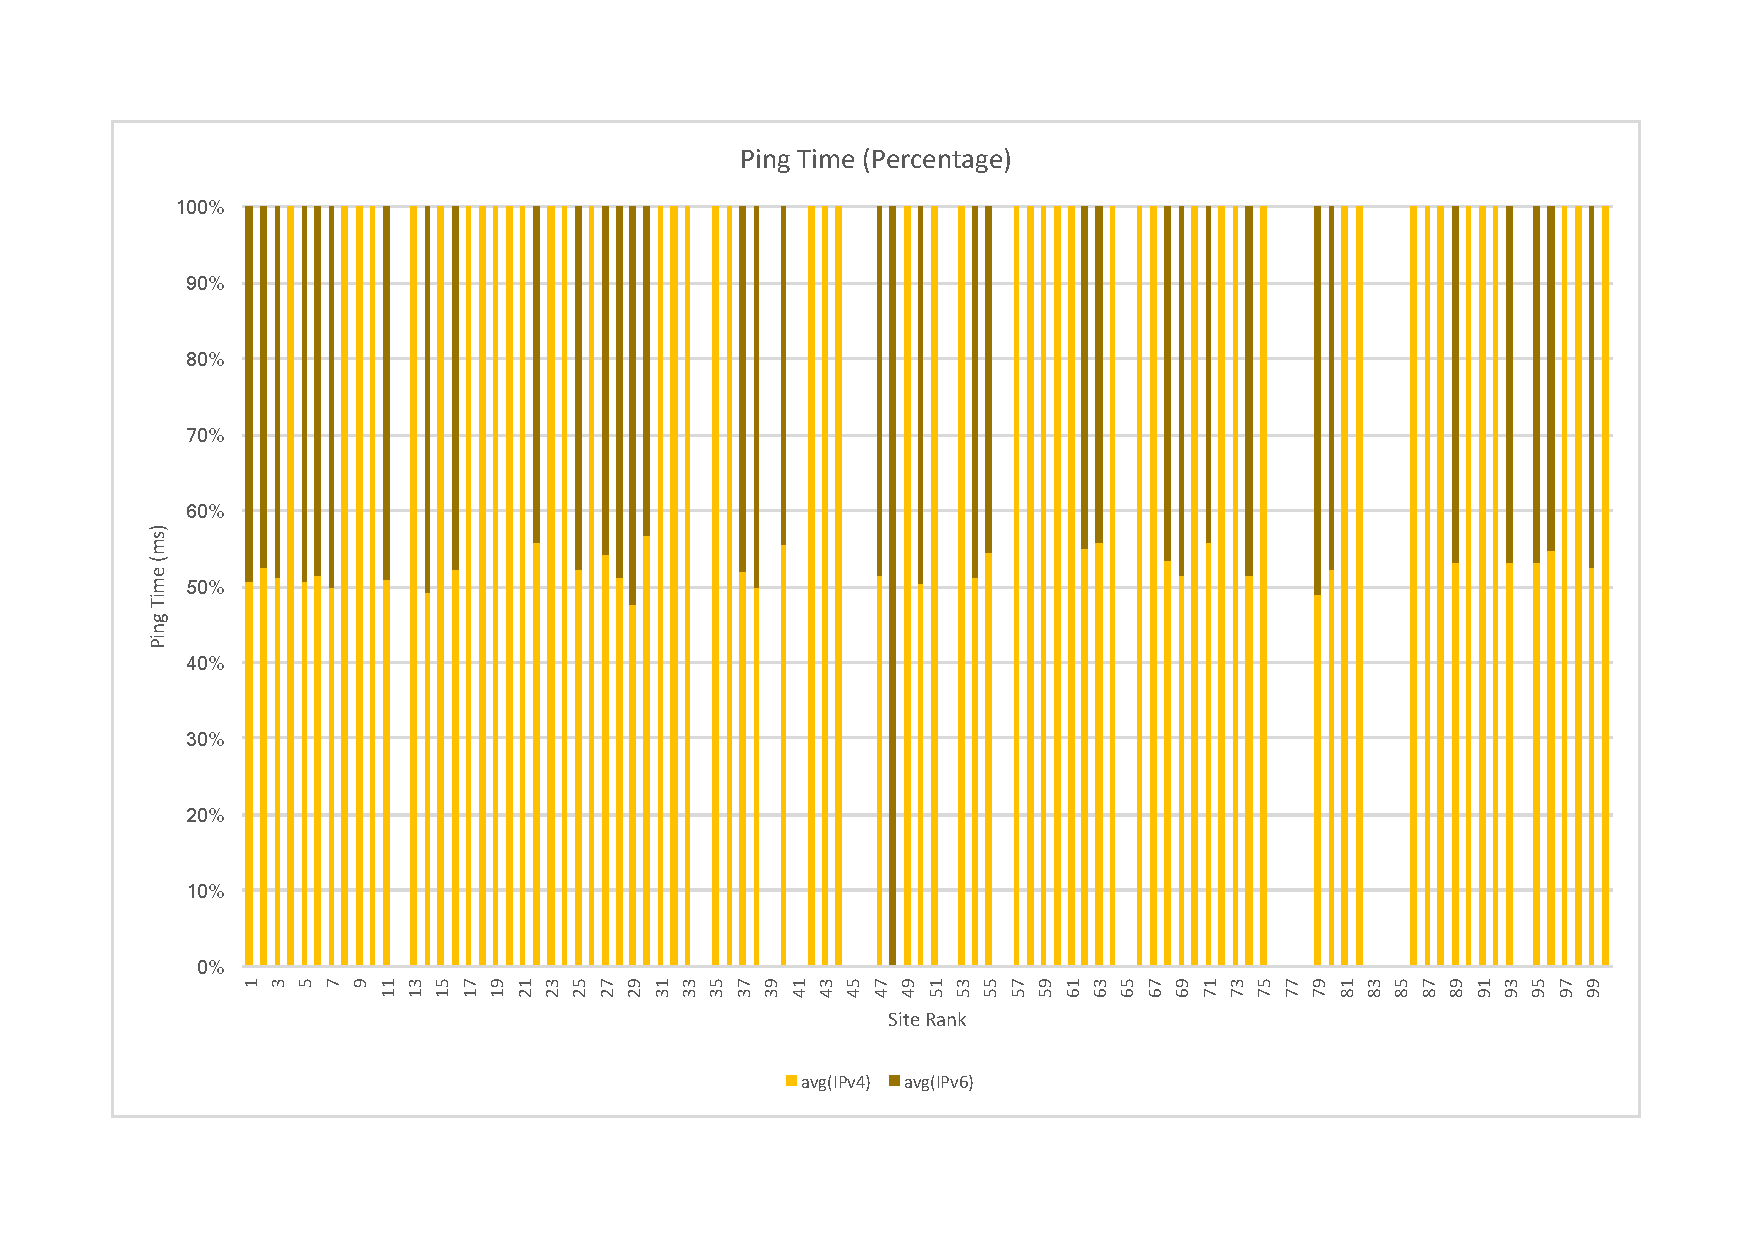
\includepdf[landscape=false,scale=0.9,angle=90,pagecommand={\subsection{Ping Time Stacked (Percentage)}\label{sec:res_stacked_percentage}}]{charts/stacked_percentage.pdf}


%%
%% SECTION: Discussion
%%
\section{Discussion}
\subsection*{Results Analysis}

As shown in \Fref{sec:res_breakdown}, of all hosts, only 1\% was unreachable via {\IPF}, whereas 63\% were unable to be reached via \IPS.
Out of the 99\% of hosts reachable via \IPF, $16/99$ (16.2\%) of them blocked ping responses whereas only $1/37$ (2.7\%) blocked pings via \IPF.
The reason for the low percentage of blocked pings on {\IPS} is most probably due to the fact that the sites blocking {\IPF} pings aren't {\IPS} enabled yet.
For example \texttt{office.com} is the only site accessible from both {\IPF} and {\IPS}, and blocks pings from both protocols.

\Fref{sec:res_ipv4} and \Fref{sec:res_ipv6} shows the average, minimum and maximum pings for all 100 hosts.
It is quite interesting to see the range between minimum and maximum.
Overall, there is no definite trend, however it is evident that the higher the average, the higher the maximum and minimum pings are.
This is most likely due to geographic location.
But it appears that the higher the average ping, the greater the range of pings ($ \textrm{max} - \textrm{min}$).
I presume this is due to an increase in geographic distance, and therefore and increase in available routes to the hosts -
  some of which are massively slower than others - and what routes are currently congested at the time of sending the ping.

Overall, there is no trend in {\IPF}/{\IPS} ping times down the top 100 list.
This is most probably due to the fact that different sites are popular in different countries.
For example, even though \texttt{baidu.com} is the \nth{4} most popular site, its average ping ranks it \nth{73}.
All the IP addresses pinged (\texttt{111.13.101.208}, \texttt{123.125.114.144}, \texttt{180.149.132.47} \& \texttt{220.181.57.217})
  indicate that their servers are hosted in China.\footcite{ip_location}
This means it is physically impossible to be quick due to the physical, geographic distance the packets have to travel.
Coincidentally, the minimum geographic ping time to China is approximately \SI{50}{\milli\second} (there and back).
Add to that, the number of hops (and therefore machines handling the ping packet) is at least 18 (using \texttt{traceroute}).
The time taken to reach China and back is going to take a long time.

The graph shown in \Fref{sec:res_stacked_percentage} takes the {\IPF} and {\IPS} time and displays them as a percentage bar.
It shows that most sites that support {\IPS} and {\IPF} respond quicker via {\IPS} than they do via {\IPF}.
This slight (but barely noticeable) decrease in time could be due to how {\IPS} was designed.
Some features of {\IPS} that could result in a decrease in time include reduced fragmentation and the lack of NAT.
Reduced fragmentation means packet fragmentation is decided at the sender which means each hop does not have to reassemble packets and fragment them again.

\subsection*{Accuracy and Limitations}
Due to the amount of times the tester was run, the different locations the tests where run, and the elimination of anomalous results I believe that my results are accurate.

The nature of the methodology does not give much to indicate a website's raw performance.
The latency of a connection (ping time) is a small fraction of the time that goes into a web request.
Take \texttt{HTTP} for example. Assuming no caching of resources is occurring, \texttt{HTTP} requires:
\begin{enumerate*}
  \item A DNS lookup
  \item Making an initial connection
  \item Connecting via SSL (if applicable)
  \item Upload the request
  \item Waiting for the remote server to generate the content
  \item Download the response
\end{enumerate*}.
All of this requires a lot of time in comparison to the small(er) latencies.
It is agreed though, that the greater the latency between two computers, the longer the time taken to load content would be.
However, there are certain situations where this could be disproved.
For example, a server on a LAN could have a ping \textless \SI{1}{\milli\second}, however, the application server response time could be upward of minutes
depending on the time taken to execute scripts/generate content.

Overall, ping testing is a limited metric that cannot be used solely to identify the performance of a network connected computer.
It is more a metric to be used with other metrics to build a full picture of a computer's performance.
\end{document}
